% Source: graduate-coursework/Research/How_to_write/00_Contrastive_Synthesis.tex
% Description: Positioning of writing theories along the individual--social axis. Theories on the left locate writing primarily in the individual mind or self; theories on the right locate it in social systems. Flower's 1994 revision (dashed arrow) shifted cognitive process theory toward the social pole.

\documentclass[border=4pt]{standalone}
\usepackage{newtxtext,newtxmath}
\usepackage{tikz}
\usetikzlibrary{arrows.meta,positioning,shapes.geometric,calc,decorations.pathreplacing}

\definecolor{garnet}{HTML}{73000A}
\definecolor{atlantic}{HTML}{466A9F}
\definecolor{congaree}{HTML}{1F414D}
\definecolor{horseshoe}{HTML}{65780B}
\definecolor{rose}{HTML}{CC2E40}
\definecolor{honeycomb}{HTML}{A49137}
\definecolor{warmgrey}{HTML}{676156}
\definecolor{black90}{HTML}{363636}
\definecolor{black70}{HTML}{5C5C5C}
\definecolor{black50}{HTML}{A2A2A2}
\definecolor{black30}{HTML}{C7C7C7}
\definecolor{black10}{HTML}{ECECEC}
\definecolor{sandstorm}{HTML}{FFF2E3}

\begin{document}
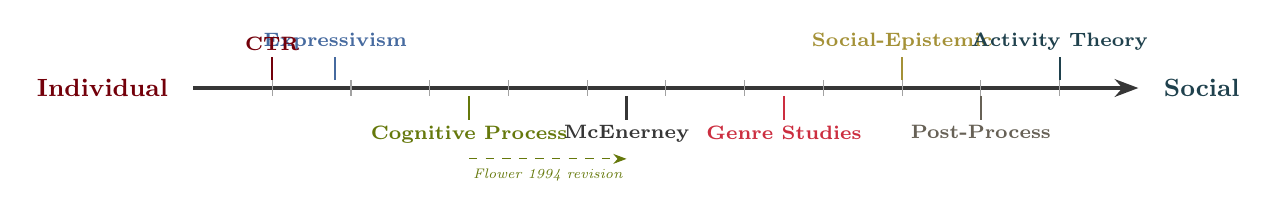
\begin{tikzpicture}[
    every node/.style={font=\footnotesize},
    theorymark/.style={font=\scriptsize\bfseries, inner sep=2pt},
]

% Individual vs Social axis
\draw[very thick, black90, -{Stealth[length=3mm]}] (-6,0) -- (6,0);
\node[font=\small\bfseries, text=garnet, anchor=east] at (-6.2,0) {Individual};
\node[font=\small\bfseries, text=congaree, anchor=west] at (6.2,0) {Social};

% Scale ticks
\foreach \x in {-5,-4,...,5} {
    \draw[black50] (\x,-0.1) -- (\x,0.1);
}

% Theory positions
\node[theorymark, text=atlantic, above=0.4cm] at (-4.2,0) {Expressivism};
\draw[thick, atlantic] (-4.2,0.1) -- (-4.2,0.4);

\node[theorymark, text=horseshoe, below=0.4cm] at (-2.5,0) {Cognitive Process};
\draw[thick, horseshoe] (-2.5,-0.1) -- (-2.5,-0.4);

\node[theorymark, text=garnet, above=0.4cm] at (-5,0) {CTR};
\draw[thick, garnet] (-5,0.1) -- (-5,0.4);

\node[theorymark, text=rose, below=0.4cm] at (1.5,0) {Genre Studies};
\draw[thick, rose] (1.5,-0.1) -- (1.5,-0.4);

\node[theorymark, text=honeycomb, above=0.4cm] at (3,0) {Social-Epistemic};
\draw[thick, honeycomb] (3,0.1) -- (3,0.4);

\node[theorymark, text=warmgrey, below=0.4cm] at (4,0) {Post-Process};
\draw[thick, warmgrey] (4,-0.1) -- (4,-0.4);

\node[theorymark, text=congaree, above=0.4cm] at (5,0) {Activity Theory};
\draw[thick, congaree] (5,0.1) -- (5,0.4);

\node[theorymark, text=black90, below=0.4cm] at (-0.5,0) {McEnerney};
\draw[thick, black90] (-0.5,-0.1) -- (-0.5,-0.4);

% Flower's revision arrow
\draw[-{Stealth}, thin, horseshoe, dashed] (-2.5,-0.9) -- (-0.5,-0.9);
\node[font=\tiny\itshape, text=horseshoe, below] at (-1.5,-0.9) {Flower 1994 revision};

\end{tikzpicture}
\end{document}
